\documentclass[a4paper]{scrartcl}
% \usepackage[utf8]{inputenc}
\usepackage[a4paper,height=23cm]{geometry}
\usepackage{graphicx}
\usepackage{listings}
\usepackage{subfig}

%opening
\title{Explore Weather Trends}
\author{Eileen Hertwig}
\subtitle{Project 1}

\begin{document}

\maketitle

\section{Introduction}

In the following time series of global mean temperature and local temperatures in Hamburg, Germany are analyzed. 
The focus of this study is on temperature trends and the differences or similarities between the global mean and the local time series. 
Moving averages are applied to the data. 
A short analysis of different time intervals for the moving averages is included. 

This analysis and the conclusions depend very much on the data. 
Global mean data has to be collected from many different locations where measurements might not be taken with the same methods or the same accuracy. 
Also it has to be expected that many areas have not been covered. 
This is especially true for oceans. 
Temperature measurements have improved over time but have only become uniform in space and time since satellite data is available (approximately starting from the 1980s). 
Without knowing how the data was measured and if or how it was cleaned all results should be treated carefully. 
Furthermore, it is not known what kind of temperature is included in the data (for example surface air temperature or 2~m temperature). 

\section{Data}
\subsection{SQL Queries}
To extract the data SQL queries are used. 
First, to find the nearest city with available data, all cities in Germany are listed with the following query:
\begin{lstlisting}[language=sql]
SELECT city
FROM city_list
WHERE country='Germany';
\end{lstlisting}
\textit{Berlin}, \textit{Hamburg}, and \textit{Munich} are listed. 
Since I live in Hamburg, I choose this city to explore temperature trends. 

To extract the temperature data for Hamburg, the following query is used:
\begin{lstlisting}[language=sql]
SELECT year, avg_temp
FROM city_data
WHERE city='Hamburg';
\end{lstlisting}

The global temperature data is extracted with the following query:
\begin{lstlisting}[language=sql]
SELECT *
FROM global_data;
\end{lstlisting}

\subsection{Missing Values}
In this project the years from 1750 to 2013 are considered. 
For the city of Hamburg the time series starts 1743 but with missing values in the years 1746--1749. 
For the global mean temperature the time series starts at 1750. 
Starting from 1750 there are no missing values in both time series, so the decision to exclude the first 7 years from the Hamburg time series seems reasonable. 

For the global mean temperature the time series extends to 2015, but for Hamburg only to 2013. 
To keep it uniform, the last two years of the global mean temperature time series are excluded. 


\section{Moving Average}
Moving averages over 5, 11, 31, and 51 years are computed. 
Different averaging intervals are used to compare the differences and find the best fit. 
Here a centralized moving average is used even though in the instructions it was explained differently. 
So if an average is computed over e.g.\ 5~years, the result is assigned to the third year, so that an equal number of years before and after are used (as well as the current year of course). 
This is also the reason why only odd number of years are chosen as averaging intervals. 

The moving average has been computed with Python. 
The following function computes the moving average for an averaging interval of $n$ years for the temperature time series $data$:
\begin{lstlisting}[language=python]
 def ma(data,n):
    s = [0]
    r = []
    for i,t in enumerate(data,1):
        s.append(s[i-1]+t)
        if i >= n:
            r.append((s[i] - s[i-n])/n)
    return r

\end{lstlisting}


\section{Results}

\begin{figure}[h!]
 \centering
 \subfloat[5-year moving average]{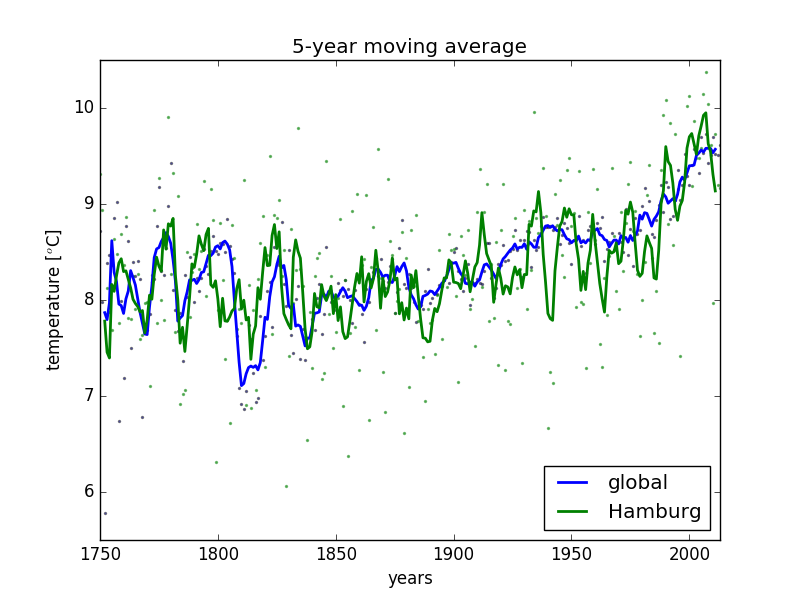
\includegraphics[width=0.45\textwidth]{MA5.png}}\qquad
 \subfloat[11-year moving average]{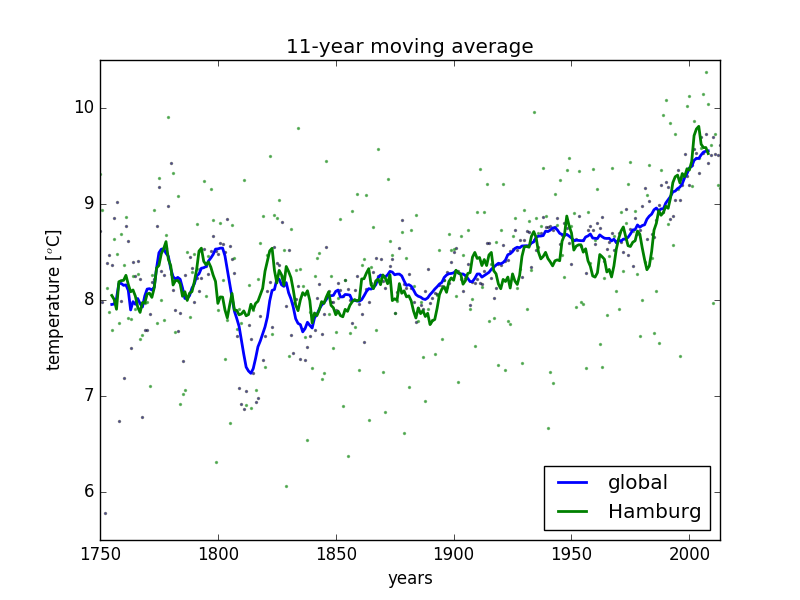
\includegraphics[width=0.45\textwidth]{MA11.png}}
 
 \subfloat[31-year moving average]{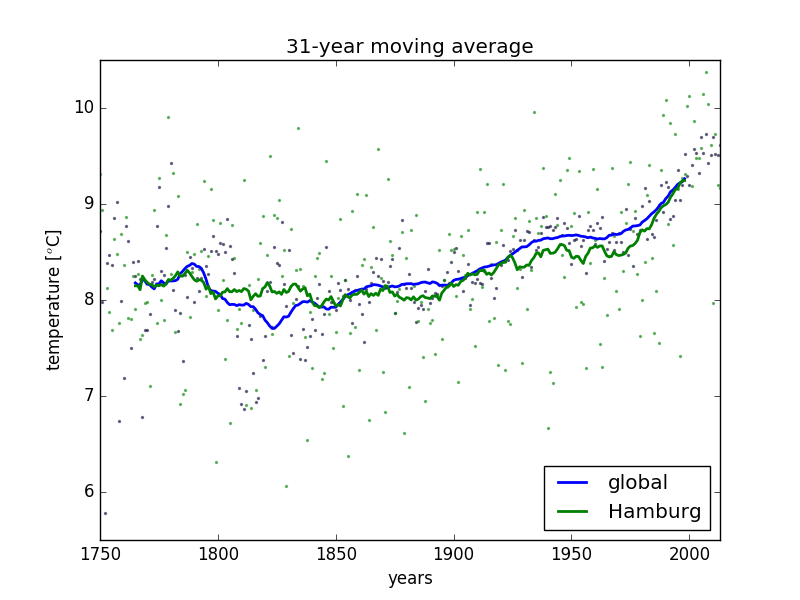
\includegraphics[width=0.45\textwidth]{MA31.png}}\qquad
 \subfloat[51-year moving average]{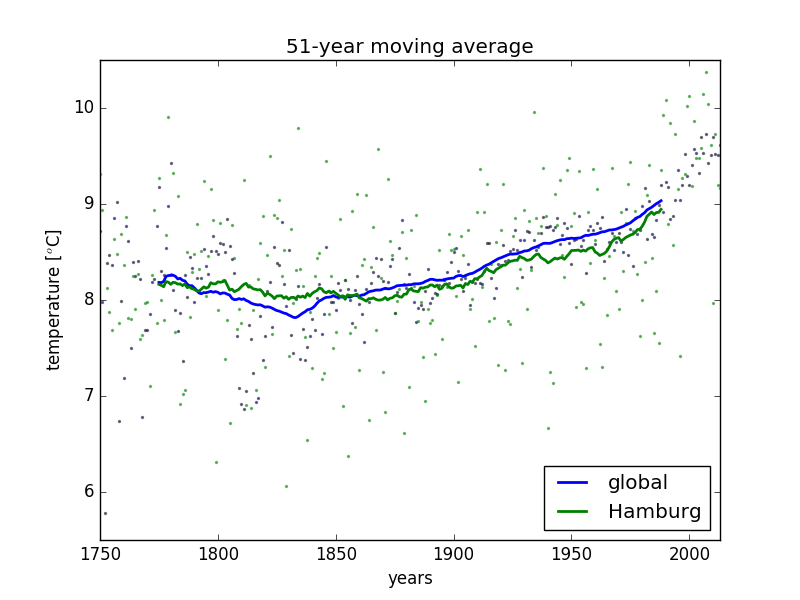
\includegraphics[width=0.45\textwidth]{MA51.png}} 
 
 \caption{Time series of the global mean temperature (blue) and the temperature for Hamburg, Germany (green). The dots are the individual yearly values while lines indicate moving averages with averaging intervals of (a) 5~years, (b) 11~years, (c) 31~years, and (d) 51~years.}
\end{figure}

Just looking at the scatter plots of the individual yearly values (dots in fig.~1) does not give a clear picture because the variability especially of the global mean temperature is very high. 
This variability is especially high in the first half of the time series. 
This can to a large extend be explained by inconsistent measurements of temperature in the $18^{th}$ and $19^{th}$ century. 
The points that indicate the temperature time series for Hamburg show less variability. 
This is mostly due to the fact that all measurements are from the same location and not averaged over the entire globe. 
Temperatures in Hamburg seem to be above the global average after 1850 and below before that time. 

To get a clearer picture of temperature trends moving averages are shown (solid lines in fig.~1). 
Often a time period of about 30~years is used to define climate. 
Fig.~1c shows the 31-year moving average. 
The first 100~years of the time series does not show a warming (since its still pre-industrial times, a warming of the global climate is not expected). 
For the global time series the 31-year running mean does not show any trends up to approximately 1900. 
In Hamburg a pronounced temperature minimum can be observed between 1800 and 1850 (which could be related to the so-called ``Little Ice Age'', which took place in the Northern Hemisphere  between the $16^{th}$ and $19^{th}$ century, for reference see for example the fourth assessment report of the IPCC\footnote{AR4, WG1 Section 6.6: The Last 2,000 Years}). 
Between 1850 and 1900 a clear positive trend in both the global mean temperature and the temperature for Hamburg are visible. 
Around 1950 the positive trends weakens but becomes very strong again in the second half of the $21^{st}$ century. 

The 31~year moving average is noisier for the global mean time series than for Hamburg. 
If the averaging period is increased even further to 51~years (see fig.~1d) both lines become very smooth. 
The warming of the global (and local) climate is still visible, but many details are smoothed out (like the very strong trend in the last decades). 
To get more details, a shorter averaging period of 11~years is shown in fig.~1b. 
Here much more variability is included, especially in the global mean time series. 
Since the Hamburg time series is still relatively smooth, a 5-year moving average is shown in fig.~1a. 
Both time series show strong variability and the very strong temperature warming in the last century can still be seen. 
However, the signal of the trends is very contaminated by noise.
If temperature trends are the main objective 5~years seem too short and 51~years too long for a moving average. 
Depending on how much detail needs to be conserved, an averaging interval between 11 and 31~years appears to be a good choice. 

\section{Conclusion}

Global mean temperature trends are visualized and compared to a local temperature time series for the city of Hamburg. 
Different moving averages reveal that periods between 11 and 31~years should be chosen to look at temperature trends. 
The main results from this study are summarized as follows:
\begin{itemize}
 \item The global mean time series shows much higher variability than the local time series. 
 \item In pre-industrial times (before 1850) climate warming does not take place and rather a cooling event can be observed that is more pronounced in the Hamburg time series. 
 \item After 1850 temperatures are higher in Hamburg than in the global mean. 
 \item Overall the positive temperature trend in Hamburg follows the global climate warming closely. 
 \item In the last decades the temperature trends have been very strong, especially in the global mean. Therefore it appears that the global mean temperature is now comparable to the mean temperature in Hamburg. 
\end{itemize}


\end{document}
\grid
\grid
